\section{Polynomial and Rational Functions}

\subsection{Quadratic Functions}
\subsubsection{Recognising the Characteristics of Parabolas}
The graph of a quadratic function is a U-shaped curve called a parabola. One important feature of the graph is that it has
an extreme point, called the vertex. If the parabola opens up, the vertex represents the lowest point on the graph, or
the minimum value of the quadratic function. If the parabola opens down, the vertex represents the highest point on the
graph, or the maximum value. In either case, the vertex is a turning point on the graph. The graph is also symmetric with
a vertical line drawn through the vertex, called the axis of symmetry. These features are illustrated here:

\begin{align*}
    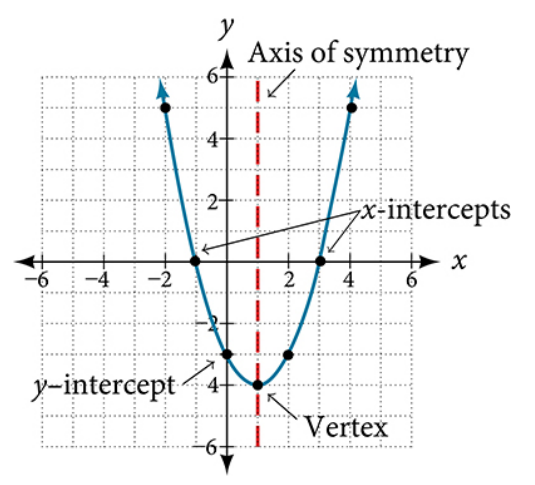
\includegraphics[width=1.1\textwidth]{algebra-pre-calculus/algebra/polynomial-and-rational-functions/parabola.png}
\end{align*}

The y-intercept is the point at which the parabola crosses the y-axis. The x-intercepts are the points at which the
parabola crosses the x-axis. If they exist, the x-intercepts represent the zeros, or roots, of the quadratic function, the
values of x for which y = 0. The x-intercepts are also called the solutions to the quadratic equation. 

\subsubsection{Understanding How the Graphs of Parabolas are Related to Their quadratic Functions}
The general form of a quadratic function presents the function in the form $f(x) = ax^2 + bx + c$. 
If $a > 0$, the parabola opens up. If $a < 0$, the parabola opens down. We can use the general form of a parabola to find the equation for the axis of symmetry.

axis of symmetry: $x = -\frac{b}{2a}$

\begin{align*}
    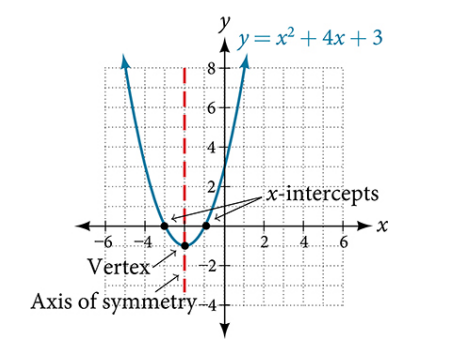
\includegraphics[width=1.1\textwidth]{algebra-pre-calculus/algebra/polynomial-and-rational-functions/parabola_example.png}
\end{align*}

The standard form of a quadratic function presents the function in the form $f(x) = a(x - h)^2 + k$.
where the vertex is at the point $(h, k)$. If $a > 0$, the parabola opens upward and the vertex is a minimum. If $a < 0$, the parabola opens downward and the vertex is a maximum.

\begin{align*}
    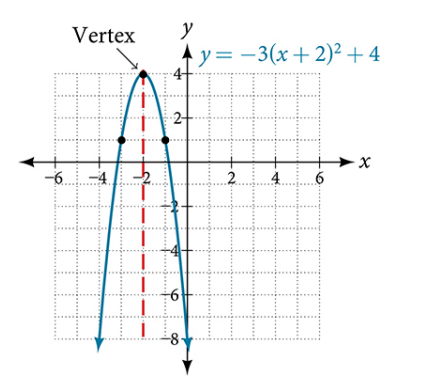
\includegraphics[width=1.1\textwidth]{algebra-pre-calculus/algebra/polynomial-and-rational-functions/vertex.png}
\end{align*}

If $k>0$ the graph shifts upward, whereas if $k<0$ the graph shifts downward. In the graph above, $k>0$ so the graph is shifted
4 units upward. If $h>0$ the graph shifts toward the right and if $h<0$ the graph shifts to the left. In the graph above, $h<0$ so
the graph is shifted 2 units to the left. The magnitude of $a$ indicates the stretch of the graph. If $|a|>1$ the point
associated with a particular x-value shifts farther from the x-axis, so the graph appears to become narrower, and there
is a vertical stretch. But if $|a|<1$, the point associated with a particular x-value shifts closer to the x-axis, so the graph
appears to become wider, but in fact there is a vertical compression. In the graph above, $|a|>1$ so the graph becomes
narrower.

\begin{align*}
    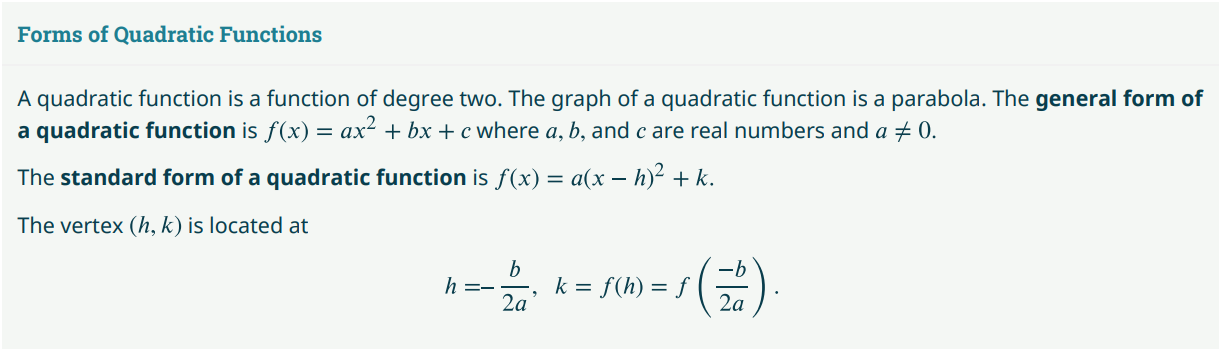
\includegraphics[width=1.1\textwidth]{algebra-pre-calculus/algebra/polynomial-and-rational-functions/quadratic_function_definition.png}
\end{align*}

The standard form and the general form are equivalent methods of describing the same function. We can see this by
expanding out the general form and setting it equal to the standard form.

\begin{align*}
    a(x - h)^2 + k &= ax^2 + bx + c \\
    a(x^2 - 2hx + h^2) + k &= ax^2 + bx + c \\
    ax^2 - 2ahx + ah^2 + k &= ax^2 + bx + c 
\end{align*}

For the linear terms to be equal, the coefficients must be equal.
$$-2ah=b$$ 
$$h=-\frac{b}{2a}$$

This is the axis of symmetry we defined earlier. Setting the constant terms equal:
$$ah^2 + k = c$$
$$k = c - ah^2$$
$$ k = c - a\left(-\frac{b}{2a}\right)^2$$
$$ k = c - \frac{b^2}{4a}$$